\chapter{Architectures}
Software architectures show the logical organizazion of a distributed system into software components, the system architecture is the final instantiation of the theoretical software architecture. \n
A couple of well known architectural styles are:
\begin{itemize}
    \item Layered
    \item Object oriented
    \item Resource orienteted
    \item Event based
\end{itemize}
Now we'll rapidly go through each of them. \n
\textbf{Layered architecture} \n
Components are organized in a layered fashion, a component can make a downcall (as in the case of calls to the operating system). \n
Upcalls are exceptions.
\smallSpace
\textbf{Object oriented architecture} \n
The components in an object oriented architecture are objects and connect to each other through procedure calls, the calls can be distributed if the objects are on different machines. \n
In the distributed case we can have separation of interfaces and objects and we can do calls via RPC. \n
Service oriented architectures are distributed applications constructed via service composition. \n
\smallSpace
\textbf{Resource base architectures} \n
A REST architecture is focused on resources and their indexing. Usually we have an interface that exposes a series of methods concerning actions we can do with respect to them. In a REST architecture:
\begin{itemize}
    \item Resources are identified through a single naming scheme
    \item All services offer the same interface
    \item Messages sent to or from service are fully self-described
    \item The communication is stateless
    \item The operations we can do with resources are a few and are standard.
\end{itemize}
When building a software architecture we are in front of two very different structures. Centralized organization, in which we have a server offering and a client recieving, the communication is of type request reply. \n
An example of centralized organization is a multitiered architecture, in which we have a client and one or more servers handling different aspects of the service (as an example: the MVC architecture, where we have a division between Model (data), View (frontend), Control (backend)). \n
When working with a multitiered architecture we can use two different models:
\begin{itemize}
    \item Vertical distribution: We divide the distributed applciation into three logical layers and we run the components from each layer on a different server.
    \item Horizontal distribution: A client or server can be physically split up into logically equivalent parts. Each part is operating on its own share of the complete data set (balancing the load).
\end{itemize}
The opposite of Centralized architecture is the Decentralized architecture, which are peer-to-peer architectures. \n
In peer-to-peer systems each node of the network is considered on the same level of the others, each of them can access data possessed by other nodes in the network and share its own. Not all peer-to-peer are built the same, it can be:
\begin{itemize}
    \item Structured: it's an overlay that adheres to a specific topology and uses a semantic-free index where each data item is uniquely associated with a key. For lookup we use a distributed hastable.
    \item Unstructured: In which we have an ad-hoc list of neighbours, to search data we can either flood the network or do a random walk.
    \item Hierarchically organized: We have a super peer which acts like an orchestrator, an index server and brokers to decide where to store data. An example of this is a Content Delivery Network.
\end{itemize}
Like with everything it's not always either black or white, we have hybrid architectures in which we combine a decentralized architecture with the client-server archetipe. \n
An example of hybrid architecture is the \textbf{Edge-server architecture} which uses client-server to manage the connection between private networks placed outside of internet's bounds and use an orchestrator or an edge server to communicate with the world. \n
Another example are collaborative distributed systems like Emule, bitTorrent, et al...
\begin{figure}[htb]
    \centering
    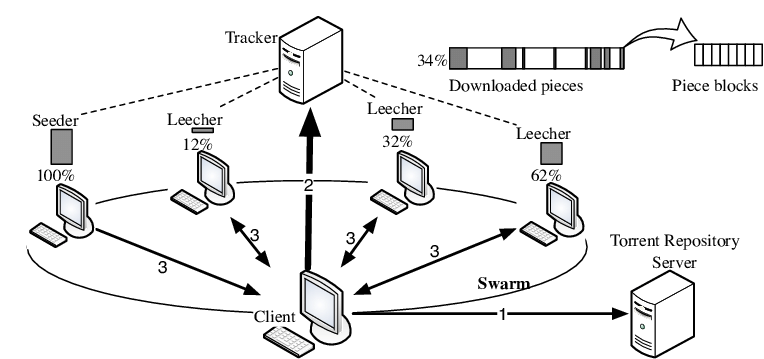
\includegraphics[scale=0.45]{img/bittorrent.png}
    \caption{Structure of the bitTorrent network}
\end{figure}
